\textbf{Входные параметры:}
 
 VectorOfProbability --- массив вероятностей выбора индивидов для порпоциональной селекции;
 
 VMHL\_N --- размер массива пригодностей.

\textbf{Возвращаемое значение:} 

Номер выбранной пригодности, а, соответственно, номер индивида популяции.

 \textbf{Принцип работы:}

\begin{figure} [h]
  \center
  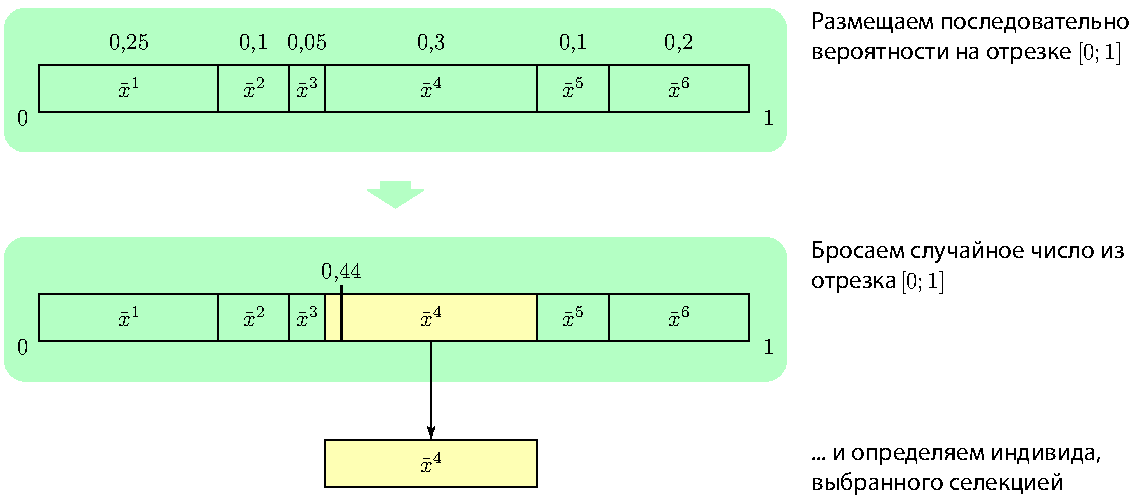
\includegraphics [scale=0.8] {MHL_ProportionalSelection_Sheme}
  \caption{Механизм работы пропорциональной селекции} 
  \label{img:MHL_ProportionalSelection_Sheme}  
\end{figure}

\textbf{Примечание:}

Связка данной функции и MHL\_MakeVectorOfProbabilityForProportionalSelectionV2 аналогична по действию (результат действия аналогичен):
 
 \begin{enumerate}
\item Функции MHL\_ProportionalSelection;
\item Функции MHL\_ProportionalSelectionV3.
 \end{enumerate}
 
 Различия по временным затратам на выполнение. У этой связки выполнение быстрее, чем у MHL\_ProportionalSelection.
  
\textbf{О функции:}

 Данная функция используется в стандартном генетическом алгоритме, реализованным в виде функции MHL\_StandartGeneticAlgorithm. Работает в связке с функцией MHL\_MakeVectorOfProbabilityForProportionalSelectionV2. Оператор селекции работает с массивом пригодностей индивидов, но непосредственно пропорциональная селекция выбирает индивида исходя из вероятностей выбора индивидов. Каждый раз для выбора индивида создавать массив вероятностей затратно, поэтому для каждой популяции на каждом поколении вначале вызывается функция MHL\_MakeVectorProbabilityForSelectionProportionalV2 для генерации вектора вероятностей выбора индивида, а затем этот массив и подставляется в пропорциональную селекцию.

